\section{Equazione di Dirac}
Le due equazioni: Klein-Gordon e Dirac sebbene soffrano del paradosso di Klain e non permettono di dare una descrizione soddisfacente in meccanica quantistica relativistica ma sono importantissime in quanto vengono integrate nella QFT. Avviene quella che è chiamata come seconda quantizzazione. La prima difficoltà dell'equazione di Kelin-Gordon è stata l'apparizione di una densità di probabilità negativa dovuta dalla derivata seconda rispetto al tempo. Dirac quindi affrontò il problema in modo diretto richiedendo:
\begin{enumerate}
    \item Un'equazione di primo grado rispetto al tempo;
    \item Anche di primo grado rispetto alle coordinate spaziali (è necessario che questa equazione sia relativisticamente covariante e quindi tutte le coordinate vanno trattate allo stesso modo);
    \item Che comunque riproducesse la corretta relazione $E^2=\mathbf{p}^2+m^2$. Il che è equivalente a richiedere che la funzione d'onda $\psi$ sia anche soluzione dell'equazione di Klein-Gordon;
    \item Inoltre l'equazione deve essere invariante per trasformazioni di Lorentz.
\end{enumerate}
Con queste premesse Dirac fece un ragionamento piuttosto semplice e ipotizzò che l'equazione dovesse avere la seguente forma:
\begin{equation}
    \begin{gathered}i \frac{\partial}{\partial t} \psi=\left[-i\left(\alpha_1 \frac{\partial}{\partial x_1}+\alpha_2 \frac{\partial}{\partial x_2}+\alpha_3 \frac{\partial}{\partial x_3}\right)+\beta m\right] \psi \\ i \frac{\partial}{\partial t} \psi=\left[-i \sum_k \alpha_k \frac{\partial}{\partial x_k}+\beta m\right] \psi\end{gathered}
\end{equation}
Questa rappresenta l'equazione più generale possibile a coefficienti costanti. Identifichiamo l'Hamiltoniana dell'equazione di Dirac:
\begin{equation*}
    i \frac{\partial}{\partial t} \psi=\left[-i \sum_k \alpha_k \frac{\partial}{\partial x_k}+\beta m\right] \psi \quad H=-i \sum_k \alpha_k \frac{\partial}{\partial x_k}+\beta m \quad H = -i\boldsymbol{\alpha} \cdot\mathbf{\nabla}+\beta m
\end{equation*}
Ritrovando l'equazione di Schr\"odinger:
\begin{equation*}
    i\frac{\partial }{\partial t}\psi=H\psi
\end{equation*}
Per completezza, scriviamo anche l'equazione di Dirca in forma estesa quando $\hbar$ e $c$ sono diversi da $1$:
\begin{equation}
    i\hbar \frac{\partial}{\partial t} \psi=\left[-i\hbar c \sum_k \alpha_k \frac{\partial}{\partial x_k}+\beta mc^2\right] \psi
\end{equation}
Per determinare la natura delle grandezze $\boldsymbol{\alpha}$ e $\beta$ richiediamo il punto $3$ (soddisfare l'equazione di Klein-Gordon). Applichiamo $i\partial/\partial t$ all'equazione di Dirac:
\begin{equation*}
    i \frac{\partial}{\partial t} i \frac{\partial}{\partial t} \psi = i \frac{\partial}{\partial t} H \psi \qquad -\frac{\partial^2}{\partial t^2} \psi = H i \frac{\partial}{\partial t} \psi \qquad -\frac{\partial^2}{\partial t^2} \psi = H H \psi
\end{equation*}
Introducendo la forma esplicita dell'Hamiltoniana
$$
-\frac{\partial^2}{\partial t^2}\psi = \left[ -i \sum_k \alpha_k \frac{\partial}{\partial x_k} + \beta m \right] \left[ -i \sum_l \alpha_l \frac{\partial}{\partial x_l} + \beta m \right] \psi
$$
Sviluppando il prodotto (facendo attenzione all'ordine nei prodotti):
$$
-\frac{\partial^2}{\partial t^2}\psi = \left\{ -\sum_k \alpha_k \frac{\partial}{\partial x_k} \sum_l\alpha_l \frac{\partial}{\partial x_l} - i m \sum_k \alpha_k \beta \frac{\partial}{\partial x_k} - i m \sum_l \beta \alpha_l \frac{\partial}{\partial x_l} + \beta^2 m^2 \right\} \psi
$$
Raccogliamo i termini "diagonali" e i termini "incrociati" separatamente
$$
-\frac{\partial^2}{\partial t^2}\psi = \left\{ -\sum_k \alpha_k^2 \frac{\partial^2}{\partial x_k^2} -\sum_{\substack{k,l=1 \\ k>l}}^3 (\alpha_k \alpha_l + \alpha_l \alpha_k) \frac{\partial}{\partial x_k} \frac{\partial}{\partial x_l} - i m \sum_k (\alpha_k \beta + \beta \alpha_k) \frac{\partial}{\partial x_k} + \beta^2 m^2 \right\} \psi
$$
per ritrovare l'equazione di Klein-Gordon fissiamo condizioni su $\alpha_k$ e $\beta$, infatti ho termini lineari nelle derivate, non ho derivate miste e anche il termine di derivate con la massa non c'è:
$$
\alpha_k^2 = 1 \qquad \alpha_k \alpha_l + \alpha_l \alpha_k = 0 \quad k \ne l \qquad \alpha_k \beta + \beta \alpha_k = 0 \qquad \beta^2 = 1
$$
Per soddisfare queste relazioni le quantità $\alpha_k$ e $\beta$ non devono commutare e pertanto esse devono per forza di cose essere matrici.
\section{Proprietà delle matrici alfa e beta}
Le relazioni appena trovate sono espresse più convenientemente introducendo l'anticommutatore di due matrici A e B: $\left\{A,B\right\}=AB+BA$:
\begin{equation}
    \left\{\alpha_j,\alpha_k\right\}=2\delta_{jk}\hat{1}\qquad \left\{\alpha_j,\beta\right\}=\hat{0} \qquad \beta^2=\hat{1}
\end{equation}
Determiniamo alcune proprietà delle matrici $\alpha$ e $\beta$. Infatti, devono essere hermitiane (in quanto l'Hamiltoniana H deve essere hermitiana e $i\nabla$ è un operatore hermitiano)
\begin{equation*}
    H=-i\boldsymbol{\alpha}\cdot\mathbf{\nabla}+\beta m
\end{equation*}
Dal momento che $\alpha^2=\beta^2=1$ gli autovalori (reali) devono essere $\lambda=\pm1$:
\begin{equation*}
    \beta u=\lambda u \quad \beta^2u=\lambda\beta u=\lambda^2u \qquad u=\lambda^2u \quad \lambda^2=1 \quad \lambda=\pm1
\end{equation*}
Sono matrici con traccia nulla. Sfruttiamo la proprietà ciclica della traccia $Tr\left[ABC\right]=Tr\left[CAB\right]$, abbiamo pertanto che:
\begin{equation*}
    Tr[\alpha_k]=Tr\left[\beta^2\alpha_k\right]=-Tr\left[\beta\alpha_k\beta\right]=-Tr\left[\beta^2\alpha_k\right]=-Tr\left[\alpha_k\right]
\end{equation*}
Concludiamo che:
\begin{equation*}
    Tr\left[\alpha_k\right]=0 \qquad Tr\left[\beta_k\right]=0 
\end{equation*}
Le matrici hanno un rango pari infatti se c'è traccia nulla e autovalori $\pm1$ implicano che il rango deve essere pari. Abbiamo 4 matrici pertanto il valore minimo del rango è 4. Infatti le matrici $(2\times2)$ di Pauli hanno le proprietà richiesta ma sono solo 3:
\begin{equation*}
    \sigma_1 = \begin{pmatrix} 0 & 1 \\ 1 & 0 \end{pmatrix} \qquad \sigma_2 = \begin{pmatrix} 0 & -i \\ i & 0 \end{pmatrix} \qquad \sigma_3 = \begin{pmatrix} 1 & 0 \\ 0 & -1 \end{pmatrix}
\end{equation*}
Pertanto le matrici $\alpha$ e $\beta$ hanno dimensione $4\times4$. Quindi anche la funzione d'onda $\psi$ ha 4 componenti MA NON è UN QUADRIVETTORE DI LORENTZ. Infatti viene detto spinore:
\begin{equation*}
    \psi = \begin{pmatrix} \psi_1 \\ \psi_2 \\ \psi_3 \\ \psi_4 \end{pmatrix}
\end{equation*}
Ci sono infinite possibilità per le matrici $\alpha$ e $\beta$. Legate fra loro da trasformazioni unitarie $\alpha'=U\alpha U^{-1}$. Ne considereremo solo 2:
\begin{itemize}
    \item La rappresentazione di Pauli-Dirac che è molto utile per studiare l'appossimazione non relativistica. Vedremo anche che in questo limite si recupera l'equazione di Schr\"odinger.
    \item La rappresentazione di Weyl o rappresentazione Chirale che serve nel limite ad alta energia o massa della particella nulla.
\end{itemize}
In moltissimi casi comunque non è necessario scrivere esplicitamente le matrici.
\section{Rappresentazione di Pauli-Dirac}
Nella Rappresentazione di Pauli-Dirac le matrici sono:
\begin{equation*}
    \alpha_k = \begin{pmatrix} \hat{0} & \sigma_k \\ \sigma_k & \hat{0} \end{pmatrix} \qquad \beta = \begin{pmatrix} \hat{1} & \hat{0} \\ \hat{0} & -\hat{1} \end{pmatrix} \qquad \hat{1} = \begin{pmatrix} \hat{1} & 0 \\ 0 & \hat{1} \end{pmatrix}
\end{equation*}
In questa forma (a blocchi) le quantità $\hat{1}$ e $\hat{0}$ sono matrici di dimensione $2\times 2$. Ricordiamo alcune proprietà delle matrici di Pauli $\sigma$
\begin{equation*}
    \left\{\sigma_k,\sigma_l \right\}=2I\delta_{kl} \qquad \left[\sigma_k,\sigma_l\right]=2i\varepsilon_{klm}\sigma_m
\end{equation*}
quindi:
\begin{equation*}
    \sigma_k\sigma_l=-\sigma_l\sigma_k=i\sigma_m
\end{equation*}
\begin{equation*}
    \sigma_k\sigma_l=i\sum_m\varepsilon_{klm}\sigma_m
\end{equation*}
La proprietà del commutatore si può anche scrivere (k,l,m ciclici).
Si dimostra che:
\begin{equation*}
    \left(\boldsymbol{\sigma}\cdot\mathbf{a}\right)\left(\boldsymbol{\sigma}\cdot\mathbf{b}\right)=\mathbf{a}\cdot\mathbf{b}\hat{1}+i\boldsymbol{\sigma}\cdot\left(\mathbf{a}\times\mathbf{b}\right)
\end{equation*}
\begin{equation*}
    \exp{\left[i\alpha\hat{\mathbf{n}}\cdot\boldsymbol{\sigma}\right]}=\hat{1}\cos{\alpha}+\hat{\mathbf{n}}\cdot\boldsymbol{\sigma}\sin{\alpha}
\end{equation*}
\section{Soluzione dell'equazione di Dirac: Onde Piane}
Cerchiamo una soluzione del tipo (onda piana). Abbiamo detto che $\psi$ deve essere uno spinore quindi $w$ è uno spinore:
\begin{equation*}
    \psi(x)=we^{-ip\cdot x}
\end{equation*}
Nella soluzione $x$ e $p$ sono $4-$vettori e $w$ è uno spinore. Inoltre abbiamo costruito l'equazione di Dirac in modo che $\psi$ soddisfi anche l'equazione di Klein-Gordon e pertanto deve essere:
\begin{equation*}
    p^2=p^2_0-\mathbf{p}^2=m^2
\end{equation*}
Sostituendo nell'equazione di Dirac:
\begin{equation*}
    i \frac{\partial}{\partial t} \psi=\left[-i \sum_k \alpha_k \frac{\partial}{\partial x_k}+\beta m\right] \psi
\end{equation*}
Otteniamo l'equazione matriciale 
\begin{equation*}
    p_0w=\left(\boldsymbol{\alpha}\cdot\mathbf{p}+\beta m\right)w=Hw \qquad H=\boldsymbol{\alpha}\cdot\mathbf{p}+\beta m
\end{equation*}
Dove ricordiamo che:
\begin{equation*}
    p_0=\pm\sqrt{\mathbf{p}^2+m^2}=\pm E_\mathbf{p} \qquad E_\mathbf{p}=\sqrt{\mathbf{p}^2+m^2}>0
\end{equation*}
Gli spinori $w$ sono gli autovettori dell'equazione agli autovalori $Hw=p_0w$. L'Hamiltoniana $H$ è hermitiana. Quindi gli autovalori $\pm p_0$ sono $4$ e sono reali. Gli autovettori $w$ sono ortogonali. Utilizziamo ora la rappresentazione di Pauli-Dirac per le matrici $\alpha$ introducendo la rappresentazione a blocchi anche per lo spinore $w$:
\begin{equation*}
    w=\begin{pmatrix}
        \phi \\ \chi
    \end{pmatrix}
\end{equation*}
Le quantità $\phi$ e $\chi$ sono spinodi di Pauli (dimensione 2). Introducendo nell'equazione:
\begin{equation*}
    p_0w=\left(\boldsymbol{\alpha}\cdot\mathbf{p}+\beta m\right)w
\end{equation*}
Si ottiene l'equazione:
\begin{equation*}
    p_0 \begin{pmatrix} \phi \\ \chi \end{pmatrix} = \begin{pmatrix} 0 & \boldsymbol{\sigma} \cdot \mathbf{p} \\ \boldsymbol{\sigma} \cdot \mathbf{p} & 0 \end{pmatrix} \begin{pmatrix} \phi \\ \chi \end{pmatrix} + m \begin{pmatrix} \hat{1} & 0 \\ 0 & -\hat{1} \end{pmatrix} \begin{pmatrix} \phi \\ \chi \end{pmatrix}
\end{equation*}
Dalla quale si ottengono le equazioni accoppiate per $\phi$ e $\chi$
\begin{align*}
    (p_0 - m)\phi = \boldsymbol{\sigma} \cdot \mathbf{p} \chi \qquad &\Longrightarrow \qquad \phi = \frac{\boldsymbol{\sigma} \cdot \mathbf{p}}{p_0 - m} \chi \\
    (p_0 + m)\chi = \boldsymbol{\sigma} \cdot \mathbf{p} \phi \qquad &\Longrightarrow \qquad \chi = \frac{\boldsymbol{\sigma} \cdot \mathbf{p}}{p_0 + m} \phi
\end{align*}
Bisogna notare che le due equazioni non sono indipendenti. Applicando l'operatore $\boldsymbol{\sigma}\cdot\mathbf{p}/(p_0+m)$ alla prima equazione $(\phi=\boldsymbol{\sigma}\cdot\mathbf{p}/((p_0+m)\chi)$
\begin{equation*}
    \frac{\boldsymbol{\sigma}\cdot\mathbf{p}}{p_0+m}\phi=\frac{\boldsymbol{\sigma}\cdot\mathbf{p}}{p_0+m}\frac{\boldsymbol{\sigma}\cdot\mathbf{p}}{p_0-m}\chi \qquad (\boldsymbol{\sigma}\cdot\mathbf{p})^2=\mathbf{p}^2
\end{equation*}
Ritrovo la seconda equazione
\begin{equation*}
    \frac{\boldsymbol{\sigma}\cdot\mathbf{p}}{p_0+m}\phi=\frac{\mathbf{p}^2}{p_0^2-m^2}\chi \qquad \frac{\boldsymbol{\sigma}\cdot\mathbf{p}}{p_0+m}\phi=\frac{\mathbf{p}^2}{\mathbf{p}^2}\chi=\chi
\end{equation*}
\subsection{Energia positiva}
Il primo gruppo di soluzioni si trova dalla seconda equazione:
\begin{equation*}
    \left(p_0+m\right)\chi=\boldsymbol{\sigma}\cdot\mathbf{p}\phi
\end{equation*}
In questo caso usiamo l'autovalore positivo: $p_0=+E_\mathbf{p}$ poi ricaviamo $\chi$ in funzione di $\phi$
\begin{equation*}
    \chi=\frac{\boldsymbol{\sigma}\cdot\mathbf{p}}{E_\mathbf{p}+m}\phi
\end{equation*}
Sostituiamo in $w$. Pertanto la soluzione è:
\begin{equation*}
    w(\mathbf{p}) = \begin{pmatrix} \phi \\ \frac{\boldsymbol{\sigma} \cdot \mathbf{p}}{E_p + m} \phi \end{pmatrix}
\end{equation*}
Lo spinore (bidimensionale) $\phi$ è arbitrario e ci sono due possibili spinori indipendenti $\phi_r$, $r=1,2$ quindi due possibili stati
\begin{equation*}
    w(\mathbf{p}, r) = \begin{pmatrix} \phi_r \\ \frac{\boldsymbol{\sigma} \cdot \mathbf{p}}{E_p + m} \phi_r \end{pmatrix}
\end{equation*}
Una possibile scelta è data da
\begin{equation*}
    \phi_1=\begin{pmatrix}
        1\\0
    \end{pmatrix}\qquad \phi_2=\begin{pmatrix}
        0\\1
    \end{pmatrix}
\end{equation*}
Se la particella ha una massa diversa da zero si può considerare il suo sistema di riposo ($\mathbf{p}=0$) nel quale si ha:
\begin{equation*}
    w(0, r) = \begin{pmatrix} \phi_r \\ 0 \end{pmatrix}
\end{equation*}
Nel sistema di riposo i due spinori sono:
\begin{equation*}
    w(\mathbf{0}, 1) = \begin{pmatrix} 1 \\ 0 \\ 0 \\ 0 \end{pmatrix} \quad w(\mathbf{0}, 2) = \begin{pmatrix} 0 \\ 1 \\ 0 \\ 0 \end{pmatrix} \qquad \text{E infine} \qquad \psi_1(x) = \begin{pmatrix} 1 \\ 0 \\ 0 \\ 0 \end{pmatrix} e^{-imt} \quad \psi_2(x) = \begin{pmatrix} 0 \\ 1 \\ 0 \\ 0 \end{pmatrix} e^{-imt}
\end{equation*}
\subsection{Energia negativa}
Il secondo gruppo di soluzioni si trova dalla prima equazione 
\begin{equation*}
    (p_0 - m)\phi = \boldsymbol{\sigma} \cdot \mathbf{p} \chi
\end{equation*}
In questo caso usiamo l'autovalore negativo: $p_0=-E_\mathbf{p}$. Ricaviamo 
$$
\phi = \frac{\boldsymbol{\sigma} \cdot \mathbf{p}}{p_o - m} \chi \qquad \phi = \frac{\boldsymbol{\sigma} \cdot \mathbf{p}}{-E_p - m} \chi \qquad \phi = \frac{-\boldsymbol{\sigma} \cdot \mathbf{p}}{E_p + m} \chi
$$
Sostituiamo in $w$ , la soluzione è pertanto:
$$
w(\mathbf{p}) = \begin{pmatrix} \frac{-\boldsymbol{\sigma} \cdot \mathbf{p}}{E_p + m} \chi \\ \chi \end{pmatrix}
$$
Lo spinore $\chi$, analogamente a prima, è arbitrario e ci sono due possibili spinori indipendenti $\chi_r$ con $r=1,2$ quindi due possibili stati:
$$
w(\mathbf{p}, r) = \begin{pmatrix} \frac{-\boldsymbol{\sigma} \cdot \mathbf{p}}{E_p + m} \chi_r \\ \chi_r \end{pmatrix} \qquad \chi_1 = \begin{pmatrix} 1 \\ 0 \end{pmatrix} \qquad \chi_2 = \begin{pmatrix} 0 \\ 1 \end{pmatrix}
$$
Se la particella ha una massa diversa da zero si può considerare il suo sistema di riposo ($\mathbf{p}=0$) nel quale si ha:
$$
w(\mathbf{0}, r) = \begin{pmatrix} 0 \\ \chi_r \end{pmatrix}
$$
$$
w(\mathbf{0}, 3) = \begin{pmatrix} 0 \\ 0 \\ 1 \\ 0 \end{pmatrix} \quad w(\mathbf{0}, 4) = \begin{pmatrix} 0 \\ 0 \\ 0 \\ 1 \end{pmatrix} \qquad \psi_3(x) = \begin{pmatrix} 0 \\ 0 \\ 1 \\ 0 \end{pmatrix} e^{+imt} \quad \psi_4(x) = \begin{pmatrix} 0 \\ 0 \\ 0 \\ 1 \end{pmatrix} e^{+imt}
$$
Qui si può intuire il vantaggio di questa rappresentazione: quando $\mathbf{p}$ diventa molto piccolo rispetto alla massa della particella (limite non relativistico) il rapporto diventa trascurabile e quindi in questo limite esiste solo uno spinore bidimensionale e l'altro sparisce. 
\subsection{Onde piane}
Abbiamo pertanto trovato $4$ soluzioni:
\begin{itemize}
    \item Due soluzione ($r=1,2$) con energia positiva:
$$
\psi_r(x) = w(\mathbf{p}, r) \exp[-iE_p + i\mathbf{p} \cdot \mathbf{x}] = w(\mathbf{p}, r) \exp[-ip \cdot x]
$$
\item Due soluzione ($r=3,4$) con energia negativa
$$
\psi_r(x) = w(\mathbf{p}, r) \exp[+iE_p + i\mathbf{p} \cdot \mathbf{x}] = \dots\dots\dots
$$
\end{itemize}
L'esponenziale con energia negativa non è in forma covariante ma si può fare lo stesso giochino fatto nella Lezione 1: $\mathbf{p}\to-\mathbf{p}$, si utilizzano pertanto gli spinori $w(-\mathbf{p},r)$ (attenzione all'ortogonalità).
$$
\psi_r(x) = w(-\mathbf{p}, r) \exp[+iE_p - i\mathbf{p} \cdot \mathbf{x}] = w(-\mathbf{p}, r) \exp[+ip \cdot x]
$$
Per evitare di scrivere gli sviluppi con argomento negativo si definiscono due spinori per l'energia positiva $u(\mathbf{p},r)$ e due spinori con l'energia negativa $v(\mathbf{p},r)$:
\begin{align*}
    u(\mathbf{p}, r) = w(\mathbf{p}, r) \qquad r=1,2 \\
    v(\mathbf{p}, r) = w(-\mathbf{p}, r+2) \qquad r=1,2
\end{align*}
Questi sono gli spinori che vengono normalmente utilizzati per descrivere le soluzioni della particella dell'equazione di Dirac e con questi si fanno i calcoli. Scrivendo $v(\mathbf{p},r)$ esplicitamente $(r=1,2)$
$$
w(\mathbf{p}, r+2) = \begin{pmatrix} \frac{-\boldsymbol{\sigma} \cdot \mathbf{p}}{E_p + m} \chi_r \\ \chi_r \end{pmatrix} \qquad v(\mathbf{p}, r) = \begin{pmatrix} \frac{\boldsymbol{\sigma} \cdot \mathbf{p}}{E_p + m} \chi_r \\ \chi_r \end{pmatrix}
$$
Se usiamo $w$ c'è il segno meno mentre se usiamo la $v$ non c'è il segno meno!
\section{Forma covariante dell'Equazione di Dirac}
Dimostreremo che l'equazione di Dirac ha la stessa forma in tutti i sistemi inerziali
\begin{equation*}
    i \frac{\partial}{\partial t} \psi=\left[-i \sum_k \alpha_k \frac{\partial}{\partial x_k}+\beta m\right] \psi
\end{equation*}
Tuttavia la forma fin qui utilizzata non è manifestamente covariante. In particolare la coordinata t appare in modo diverso dalle $x_k$. Quindi possiamo fare un trucchetto e moltiplicare l'equazione da sinistra per $\beta$
\begin{equation*}
    i\textcolor{red}{\beta} \frac{\partial}{\partial t} \psi=\left[-i \sum_k \textcolor{red}{\beta}\alpha_k \frac{\partial}{\partial x_k}+\textcolor{red}{\beta}\beta m\right] \psi
\end{equation*}
Utilizziamo il fatto che $\beta^2=\hat{1}$ e definiamo le matrici $\gamma$
\begin{equation*}
    \gamma^0=\beta \qquad \gamma^k=\beta\alpha_k
\end{equation*}
Inoltre introduciamo
$$
\partial^\mu = (\partial/\partial t, -\partial/\partial x^k) \qquad \partial_\mu = g_{\mu\nu}\partial^\nu = (\partial/\partial t, \partial/\partial x^k)
$$
Riordinando i termini otteniamo:
$$
i\gamma^\mu \partial_\mu \psi = m\psi \qquad i\slashed{\partial} \psi = m\psi
$$
è molto usata la notazione di Feynman ($a_\mu$ è un $4-$vettore) $\slashed{a}\equiv\gamma^\mu a_\mu$. Le matrici $\gamma$ soddisfano le seguenti regole di commutazione
$$
\{\gamma^\mu, \gamma^\nu\} = 2Ig^{\mu\nu}
$$
Attenzione: verificheremo che non sono (tutte) hermitiane. Infatti le matrici "spaziali" non lo sono. 

Nella rappresentazione di Pauli-Dirac la forma delle matrici è
$$
\gamma^0 = \begin{pmatrix} \hat{1} & \hat{0} \\ \hat{0} & -\hat{1} \end{pmatrix} \qquad \gamma^k = \begin{pmatrix} \hat{0} & \sigma_k \\ -\sigma_k & \hat{0} \end{pmatrix}
$$
In forma esplicita
$$\hspace*{-2cm}
\gamma^0 = \begin{pmatrix} 1 & 0 & 0 & 0 \\ 0 & 1 & 0 & 0 \\ 0 & 0 & -1 & 0 \\ 0 & 0 & 0 & -1 \end{pmatrix} \quad \gamma^1 = \begin{pmatrix} 0 & 0 & 0 & 1 \\ 0 & 0 & 1 & 0 \\ 0 & -1 & 0 & 0 \\ -1 & 0 & 0 & 0 \end{pmatrix} \quad \gamma^2 = \begin{pmatrix} 0 & 0 & 0 & -i \\ 0 & 0 & i & 0 \\ 0 & i & 0 & 0 \\ -i & 0 & 0 & 0 \end{pmatrix} \quad \gamma^3 = \begin{pmatrix} 0 & 0 & 1 & 0 \\ 0 & 0 & 0 & -1 \\ -1 & 0 & 0 & 0 \\ 0 & 1 & 0 & 0 \end{pmatrix}
$$
Vale la pena rendersi conto di quello che la forma compatta dell'equazione di Dirac significa effettivamente
\begin{equation*}\hspace*{-3cm}
    i \begin{pmatrix} 1 & 0 & 0 & 0 \\ 0 & 1 & 0 & 0 \\ 0 & 0 & -1 & 0 \\ 0 & 0 & 0 & -1 \end{pmatrix} \begin{pmatrix} \partial_0 \psi_1 \\ \partial_0 \psi_2 \\ \partial_0 \psi_3 \\ \partial_0 \psi_4 \end{pmatrix} + i \begin{pmatrix} 0 & 0 & 0 & 1 \\ 0 & 0 & 1 & 0 \\ 0 & -1 & 0 & 0 \\ -1 & 0 & 0 & 0 \end{pmatrix} \begin{pmatrix} \partial_1 \psi_1 \\ \partial_1 \psi_2 \\ \partial_1 \psi_3 \\ \partial_1 \psi_4 \end{pmatrix} + i \begin{pmatrix} 0 & 0 & 0 & -i \\ 0 & 0 & i & 0 \\ 0 & i & 0 & 0 \\ -i & 0 & 0 & 0 \end{pmatrix} \begin{pmatrix} \partial_2 \psi_1 \\ \partial_2 \psi_2 \\ \partial_2 \psi_3 \\ \partial_2 \psi_4 \end{pmatrix} + i \begin{pmatrix} 0 & 0 & 1 & 0 \\ 0 & 0 & 0 & -1 \\ -1 & 0 & 0 & 0 \\ 0 & 1 & 0 & 0 \end{pmatrix} \begin{pmatrix} \partial_3 \psi_1 \\ \partial_3 \psi_2 \\ \partial_3 \psi_3 \\ \partial_3 \psi_4 \end{pmatrix}
\end{equation*}
\begin{equation*}
   = m \begin{pmatrix} \psi_1 \\ \psi_2 \\ \psi_3 \\ \psi_4 \end{pmatrix}
\end{equation*}
Si tratta di un sistema di equazioni differenziali alle derivate parziali
$$
\begin{cases}
i[\partial_0 \psi_1 + (\partial_1 - i\partial_2)\psi_4 + \partial_3 \psi_3] = m\psi_1 \\
i[\partial_0 \psi_2 + (\partial_1 + i\partial_2)\psi_3 - \partial_3 \psi_4] = m\psi_2 \\
i[-\partial_0 \psi_3 - (\partial_1 - i\partial_2)\psi_2 - \partial_3 \psi_1] = m\psi_3 \\
i[-\partial_0 \psi_4 - (\partial_1 + i\partial_2)\psi_1 + \partial_3 \psi_2] = m\psi_4
\end{cases}
$$
Emerge quindi la potenza del formalismo e come si dimostrano teoremi e si risolvono calcoli senza passare per queste equazioni assolutamente complesse. Prima di questa notazione compatta andavano risolte passo passo. In un articolo di Fermi si vede quanto era tedioso e complesso questo procedimento!
Tornando alle soluzioni, abbiamo visto che le soluzione (onde piane) dell'equazione di Dirac:
\begin{itemize}
    \item Due funzioni con energia positiva: $u(\mathbf{p},r)e^{-ip\cdot x}$
    \item Due funzioni con energia negativa: $v(\mathbf{p},r)e^{+ip\cdot x}$
\end{itemize}
Applicando l'equazione di Dirac in forma covariante a queste soluzioni otteniamo due equazioni per gli spinori $u$ e $v$
\begin{equation*}
    i\gamma^\mu\partial_\mu\psi=m\psi
\end{equation*}
$$
\gamma^\mu p_\mu u = mu \qquad (\slashed{p} - m)u = 0 \qquad -\gamma^\mu p_\mu v = mv \qquad (\slashed{p} + m)v = 0
$$
Anticipiamo che questa differenza di segni è molto importante quando andremo a studiare il decadimento $\beta$ di una particella o antiparticella sono differenti. Violano la simmetria particella e antiparticella che deriva da questa differenza di segno.
Ricordarsi che si tratta di due equazioni matriciali. Le soluzioni sono autofunzioni delle equazioni di Dirac. Come sempre abbiamo uno spettro continuo e quindi delle funzioni non normalizzabili. Le soluzioni normalizzabili si costruiscono come pacchetti.
$$
\psi(x) = \int \frac{d^3\mathbf{p}}{(2\pi)^{3/2}} \sum_{r=1,2} \left[ b(\mathbf{p}, r) u(\mathbf{p}, r) e^{-ip \cdot x} + d(\mathbf{p}, r) v(\mathbf{p}, r) e^{+ip \cdot x} \right]
$$
Si può verificare che uno stato iniziale localizzato (ad esempio una distribuzione gaussiana $\times w(0,1)$) ha una rappresentazione che contiene sia energie positive che negative
\section{Proprietà delle matrici gamma}
Le matrici $\gamma$ hanno alcune delle proprietà delle matrici $\alpha$ e $\beta$. Hanno traccia nulla e autovalori $\pm 1$. A differenza delle matrici $\alpha$ e $\beta$ le matrici $\gamma^k$ ($k=1,2,3$) non sono hermitiane infatti:
$$
\gamma^{0\dagger} = \beta^\dagger = \beta = \gamma^0
$$
$$
\gamma^{k\dagger} = (\beta\alpha_k)^\dagger = \alpha_k^\dagger \beta^\dagger = \alpha_k \beta = -\beta \alpha_k = -\gamma^k
$$
Queste relazioni possono essere unificate
$$
\gamma^{\mu\dagger} = \gamma^0 \gamma^\mu \gamma^0
$$
Risulta molto utile anche l'aggiunto spinoriale (definito per una matrice qualsiasi, non solo per $\gamma^\mu$)
$$
\overline{\gamma^\mu} \equiv \gamma^0 \gamma^{\mu\dagger} \gamma^0 \qquad \Longrightarrow \qquad \overline{\gamma^\mu} = \gamma^\mu
$$
Proprietà dell'aggiunto spinoriale (analoghe a quelle dell'aggiunto hermitiano)
$$
\overline{AB} = \overline{B}\,\overline{A} \qquad \overline{aA + bB} = a^*\overline{A} + b^*\overline{B}
$$
va sottolineato che tutte le espressioni scritte sono matrici $4\times 4$. Vedremo che è utile definire anche l'aggiunto spinoriale per uno spinore
\begin{equation*}
    \overline{\psi}=\psi^\dagger\gamma^0
\end{equation*}
Come nel caso dell'aggiunto hermitiano si tratta di un vettore-riga:
\begin{figure}[h!]
    \centering
    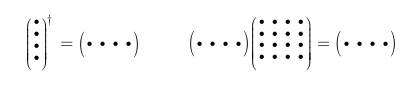
\includegraphics[width=0.8\textwidth]{Lezioni/Lezione 2/ll.png}
    \label{fig:ll}
\end{figure}
Una proprietà del prodotto di matrici $\times$ spinori
$$
A\psi \qquad \overline{A\psi} = \overline{\psi}\,\overline{A}
$$
In seguito saranno molto utili quantità scalari costruite a partire dagli spinori come ad esempio
\begin{equation*}
    \overline{u}Av
\end{equation*}
Calcoliamo il suo complesso coniugato
$$
(\overline{u}Av)^* = (u^\dagger \gamma^0 A v)^* = (u^\dagger \gamma^0 A v)^\dagger = (v^\dagger A^\dagger \gamma^{0\dagger} u) = (v^\dagger \gamma^0 \gamma^0 A^\dagger \gamma^{0\dagger} u)
$$
$$
(\overline{u}Av)^* = \overline{v}\overline{A}u = \overline{(\overline{u}Av)}
$$
\section{Corrente conservata}
Studiamo adesso come definire una corrente $j^\mu$ per l'equazione di Dirac tale che:
\begin{equation*}
    i\gamma^\mu\partial_\mu\psi=m\psi \qquad \partial_\mu j^\mu=0
\end{equation*}
Procediamo come nel caso delle equazioni di Schr\"odinger e di Klein-Gordon. Moltiplichiamo a sinistra per lo spinore aggiunto hermitiano:
$$
\psi^\dagger = (\psi_1^* \quad \psi_2^* \quad \psi_3^* \quad \psi_4^*) \qquad i\psi^\dagger \gamma^\mu \partial_\mu \psi = m\psi^\dagger \psi
$$
Scriviamo l'equazione aggiunta hermitiana
$$
(i\gamma^\mu \partial_\mu \psi = m\psi)^\dagger \quad \to \quad -i(\partial_\mu \psi)^\dagger \gamma^{\mu\dagger} = m\psi^\dagger
$$
Moltiplichiamo a destra per $\psi$ e sottraiamo alla prima equazione 
$$
i\psi^\dagger \gamma^\mu \partial_\mu \psi + i(\partial_\mu \psi)^\dagger \gamma^{\mu\dagger} \psi = m\psi^\dagger \psi - m\psi^\dagger \psi = 0
$$
Se le matrici $\gamma^\mu$ fossero hermitiane $\gamma^{\mu\dagger}=\gamma^\mu$ si potrebbe scrivere $j^\mu=\psi^\dagger\gamma^\mu\psi$ ma NON SONO HERMITIANE! Possiamo quindi utilizzare l'aggiunto spinoriale ricordando la definizione per lo spinore $\psi$
$$
\overline{\psi} = \psi^\dagger \gamma^0
$$
Ripetiamo il calcolo precedente sostituendo l'aggiunto hermitiano con l'aggiunto spinoriale. Moltiplichiamo l'equazione di Dirac a sinistra per l'aggiunto spinoriale di $\psi$
$$
\overline{\psi} = \psi^\dagger \gamma^0 \qquad i\overline{\psi}\gamma^\mu \partial_\mu \psi = m\overline{\psi}\psi
$$
Scriviamo quindi l'aggiunto spinoriale dell'equazone di Dirac
$$
\overline{i\gamma^\mu \partial_\mu \psi} = \overline{m\psi} \quad \qquad -i(\partial_\mu \psi)^\dagger \gamma^{\mu \dagger} \gamma^0 = m\psi^\dagger \gamma^0
$$
$$
-i(\partial_\mu \psi)^\dagger \textcolor{red}{\gamma^0 \gamma^0} \gamma^{\mu \dagger} \gamma^0 = m\psi^\dagger \gamma^0 \qquad -i(\partial_\mu \overline{\psi}) \overline{\gamma^\mu} = m\overline{\psi} \qquad -i(\partial_\mu \overline{\psi}) \gamma^\mu = m\overline{\psi}
$$
Moltiplichiamo a destra per $\psi$
$$
-i(\partial_\mu \overline{\psi}) \gamma^\mu \psi = m\overline{\psi}\psi
$$
e sottraiamo alla prima espressione
$$
i\overline{\psi}\gamma^\mu \partial_\mu \psi + i(\partial_\mu \overline{\psi}) \gamma^\mu \psi = m\overline{\psi}\psi - m\overline{\psi}\psi = 0
$$
$$
i\overline{\psi}\gamma^\mu \partial_\mu \psi + i(\partial_\mu \overline{\psi}) \gamma^\mu \psi = 0
$$
Il primo membro è la quadri-divergenza della corrente
$$
j^\mu = \overline{\psi}\gamma^\mu \psi \qquad \partial_\mu j^\mu = \partial_\mu (\overline{\psi}\gamma^\mu \psi) = 0
$$
Vediamo adesso se si può interpretare la corrente $j^\mu$ come densità di corrente di probabilità
$$
j^\mu = (\rho, \mathbf{j}) = (\overline{\psi}\gamma^0 \psi, \overline{\psi}\boldsymbol{\gamma} \psi)
$$
Consideriamo la densità
$$
\rho = \overline{\psi}\gamma^0 \psi = \psi^\dagger \gamma^0 \gamma^0 \psi = \psi^\dagger \psi = |\psi_1|^2 + |\psi_2|^2 + |\psi_3|^2 + |\psi_4|^2
$$
Vediamo pertanto che, a differenza di quanto avveniva per l'equazione di Klein-Gordon $\rho$ è definita positiva ed è pertanto interpretabile come densità di probabilità. Tuttavia anche l'equazione di Dirac conduce al paradosso di Klein. Occorre comunque verificare che il $4-$vettore $j^\mu$ abbia le corrette proprietà di trasformazione per una trasformazione di Lorentz. Lo vedremo in seguito.

Approfondiamo un punto legato alla normalizzazione degli spinori. Fino a questo punto non abbiamo utilizzato la possibilità di definire la normalizzazione degli spinori $w$ (o $u, v$). La quantità $\rho dV$ deve essere invariante per trasformazioni di Lorentz. L'elemento di volume $dV=dxdydz$ si contrae come $1/\gamma$ e quindi $dV\to dV/\gamma$ con $\gamma=\frac{1}{\sqrt{1-\beta^2}}$. Pertanto $\rho$ deve "dilatarsi" come $\gamma$ per compensare.
\section{Normalizzazione degli spinori}
Con un calcolo diretto si può facilmente verificare che
$$
w^\dagger(\mathbf{p}, r) w(\mathbf{p}, r) = \frac{2E_p}{E_p + m} \qquad w(\mathbf{p}, r) = \begin{pmatrix} \phi_r \\ \frac{\boldsymbol{\sigma} \cdot \mathbf{p}}{E_p + m} \phi_r \end{pmatrix}
$$
Analogamente per gli spinori di energia negativa. Pertanto se ridefiniamo la normalizzazioni degli spinori come
$$
w(\mathbf{p}, r) = \sqrt{E_p + m} \begin{pmatrix} \phi_r \\ \frac{\boldsymbol{\sigma} \cdot \mathbf{p}}{E_p + m} \phi_r \end{pmatrix}
$$
Otterremo
$$
\rho = \psi^\dagger \psi = w^\dagger(\mathbf{p}, r) w(\mathbf{p}, r) = 2E_p
$$
Ovviamente $E_\mathbf{p}$ varia come $\gamma$ ($E_\mathbf{p}=m\gamma$). Questa normalizzazione ha lo svantaggio di introdurre una dimensionalità! Inoltre ha lo svantaggio di divergere per particelle con massa nulla (come i neutrini anche se in realtà hanno massa). Per quanto riguarda l'ortogonalità degli spinori è facile verificare che gli spinori $w(\mathbf{p},r)$ sono fra loro ortogonali. Con la normalizzazione scelta $(r,q=1,4)$
$$
w^\dagger(\mathbf{p}, r) w(\mathbf{p}, q) = 2E_\mathbf{p} \delta_{rq}
$$
Per esprimere queste condizioni utilizzando gli spinori $u(\mathbf{p},r)$ e $v(\mathbf{p,r})$ bisonga essere cauti. Infatti gli spinori sono definiti come $(r=1,2)$ $v(\mathbf{p,r})=w(-\mathbf{p},r+2)$. Le condizioni di normalizzazione e ortogonalità sono pertanto $(r,q=1,2)$
$$
u^\dagger(\mathbf{p}, r) u(\mathbf{p}, q) = 2E_\mathbf{p} \delta_{rq} \qquad v^\dagger(\mathbf{p}, r) v(\mathbf{p}, q) = 2E_\mathbf{p} \delta_{rq}
$$
$$
u^\dagger(\mathbf{p}, r) v(-\mathbf{p}, q) = v^\dagger(-\mathbf{p}, r) u(\mathbf{p}, q) = 0
$$
Notiamo incidentalmente che la normalizzazione degli spinori dipende da $\mathbf{p}$ e pertanto dipende dal sistema interizale in cui si osserva lo spinore. Le trasformazioni di Lorentz per gli spinori (che introdurremo) non sono unitarie perchè non preservano la norma dello spinore.
\section{Normalizzazione usando gli aggiunti spinoriali}
Introduciamo infine le normalizzazioni degli spinori utilizzando l'operazione aggiunto spinoriale invece della coniugazione hermitiana. Ad esempio, utilizzando la forma esplicita nella rappresentazione di Pauli-Dirac
$$
u(\mathbf{p}, r) = \sqrt{E_\mathbf{p} + m} \begin{pmatrix} \phi_r \\ \frac{\boldsymbol{\sigma} \cdot \mathbf{p}}{E_p + m} \phi_r \end{pmatrix} \qquad v(\mathbf{p}, r) = \sqrt{E_\mathbf{p} + m} \begin{pmatrix} \frac{\boldsymbol{\sigma} \cdot \mathbf{p}}{E_p + m} \chi_r \\ \chi_r \end{pmatrix}
$$
Utilizzando la rappresentazione di Pauli-Dirac si dimostra facilmente che
$$
\overline{u}(\mathbf{p}, r) u(\mathbf{p}, q) = 2m\delta_{rq} \qquad \overline{v}(\mathbf{p}, r) v(\mathbf{p}, q) = -2m\delta_{rq}
$$
$$
\overline{v}(\mathbf{p}, r) u(\mathbf{p}, q) = \overline{u}(\mathbf{p}, r) v(\mathbf{p}, q) = 0
$$
Sottolineiamo che in queste relazioni la quantità di moto $\mathbf{p}$ ha sempre lo stesso segno. Si può dimostrare che queste relazioni valgono indipendentemente dalla rappresentazione. Infine questa normalizzazione è invariante rispetto al sistema di riferimento.
\section{Interpretazione delle soluzione con energia negativa}
Nella teoria di Dirac sarebbe possibile interpretare senza problemi le soluzioni con energia positiva. La densità di probabilità è definita positiva. L'evoluzione temporale (libera) di una funzione d'onda che contiene solo stati con $p_0>0$ non conduce all'apparizione di stati con $p_0<0$. Tuttavia ci sono dei problemi: da un punto di vista matematico gli autovettori dell'Hamiltoniana sono un sistema completo solo se includono anche gli stati con $p_0<0$. L'evoluzione di uno stato iniziale localizzato (ad esempio una distribuzione gaussiana) porta a stati che contengono sia energie positive che negatice. Infine se si introduce una interazione diventano possibili transizioni da stati con energia positiva a stati di energia negativa. Sarebbero, inoltre, transizioni che non assorbono energia bensì la cedono
$$
\Delta E=E_f-E_i<0
$$
Sarebbero quindi transizioni spontanee e non esisterebbero stati stabili. Dirac quindi fornì una soluzione a questi problemi. Le particelle descritte dall'equazione di Dirac sono fermioni e perciò obbediscono al principio di esclusione di Pauli. Dirac ipotizzò che, in natura, tutti gli stati con energia negativa fossero occupati da elettroni. Introdusse così un "mare" di particelle con energie negative. Il mare ha un'energia totale infinita ($E=-\infty$) e una carica infinita ($Q=-\infty$). Inoltre il mare ha un momento angolare nullo (in quanto ci sono coppie infinite di up-down). Per questo motivo non possono esserci transizioni spontanee a stati con energia negativa: tutti gli stati sono occupati! Se uno stato fisico viene descritto rispetto a questo "mare" si giunge ad una descrizione accettabile e consistente.
\begin{figure}[h!]
    \centering
    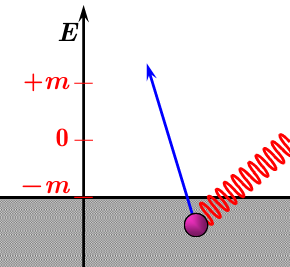
\includegraphics[width=0.4\textwidth]{Lezioni/Lezione 2/oo.png}
    \label{fig:oo}
\end{figure}
Consideriamo un sistema nel quale inizialmente ci sia solo il mare (tutti gli stati di energia negativa sono completi). Supponiamo che un fotone ceda al sistema una quantità di energia sufficiente per una transizione. Da uno stato con energia negativa $-E_k, -\mathbf{k}$ ad uno stato con energia positiva $E_p, \mathbf{p}$. Il bilancio energia-momento è:
\begin{align*}
E_\gamma + (-E_k) = E_p \quad &\Longrightarrow \quad E_\gamma = E_p + E_k \\
\mathbf{p}_\gamma + (-\mathbf{k}) = \mathbf{p} \quad &\Longrightarrow \quad \mathbf{p}_\gamma = \mathbf{p} + \mathbf{k}
\end{align*}
Nello stato finale abbiamo un elettrone di carica $-|e|$, momento $\mathbf{p}$ e spin $s$. Abbiamo creato una particella ma il mare ha perso una particella
\begin{itemize}
    \item Si è creata una buca (hole)
    \item La sua carica diminuisce di $-|e|$ mentre la carica nel mare aumenta di $|e|$
    \item La sua energia diminuisce di $(-E_k)$ mentre l'energia del mare aumenta di $E_k$
    \item Il suo momento diminuisce di $-\mathbf{k}$ mentre nel mare il momento aumenta di $\mathbf{k}$
    \item Il suo spin diminuisce di $s$ mentre lo spin del mare diventa $-s$
\end{itemize}
Abbiamo creato un'antiparticella connumeri quantici $|e|,m,E_k,\mathbf{k},-s$. Con questa interpretazione riconsideriamo gli spinori con energia negativa
\begin{equation*}
    v(\mathbf{p}, r) = \begin{pmatrix} \frac{\boldsymbol{\sigma} \cdot \mathbf{p}}{E_p + m} \chi_r \\ \chi_r \end{pmatrix}
\end{equation*}
Rappresentano una particella di massa $m$ e una carica $+|e|$. Il $4-$momento della particella è $(E_p,\mathbf{p})$. Ricordiamo che lo spinore $v(\mathbf{p}, r)$ è definito a partire dalle soluzioni $w$ con energia negativa e dalla relazione $v(\mathbf{p}, r)= w(-\mathbf{p}, r)$. Se interpretiamo  $v(\mathbf{p}, r)$ come la funzione d'onda della buca allora
\begin{itemize}
    \item Lo spinore  $v(\mathbf{p}, 1)$ rappresenta uno stato con spin down $\chi=(1\quad 0)^T$
    \item Lo spinore $v(\mathbf{p}, 2)$ rappresenta uno stato con spin up $\chi=(0\quad 1)^T$
\end{itemize}
Notare la corrispondenza fra valore "fisico" dello spin e numero dello stato. Inversa rispetto agli stati di energia positiva.